\documentclass[a4paper, 11pt]{article}
\usepackage{geometry}
\geometry{letterpaper, margin=1in}
\usepackage{amsmath}
\usepackage{amssymb}  
\usepackage{amsthm}
\usepackage{ulem} 
\usepackage{graphicx}
\graphicspath{ {images/} }

\begin{document}
%Header-Make sure you update this information!!!!
\noindent
\large\textbf{Exponential Map} \hfill \textbf{John Waczak} \\
\normalsize MTH 435 \hfill  Date: \today \\
Dr. Christine Escher \\

\subsection*{Tapp 5.21} 
	\textit{Prove Corollary 5.24. If $f:S\rightarrow \tilde{S}$ is an isometry between regular surfaces, and $\gamma$ is a geodesic in $S$, then $f\circ\gamma$ is a geodesic in $\tilde{S}$.} \\ 
	
	\noindent Since f is an isometry, it preserves distances i.e. $\forall x \in T_pS$ we have that $|x|_p = |df_p(x)|_{f(p)}$. Similarly, in our last assignment, we showed that if f is an isometry, then $d(\gamma(a), \gamma(b))=\tilde{d}(f\circ\gamma(b), f\circ\gamma(b))$.  Also, since $\gamma$ is a geodesic we have that by proposition 5.23 that $\gamma$ is locally minimizing. Thus for every segment $\{\gamma(t)|t\in[a,b]\}, \quad [a,b] \subseteq I$ it follows that:
		\begin{equation*}
			\text{length}(\gamma) = \int_a^b |\gamma'(t)|dt = d(\gamma(a), \gamma(b))
		\end{equation*}
		
	\noindent Now, since $\gamma'(t)$ is in $T_pS$ we have that the length of such a segment of this curve must be preserved under composition with f. Thus $\text{length}(\gamma)=\text{length}(f\circ\gamma)$. All that remains is to show that $\text{length}(f\circ\gamma)=d(f\circ\gamma(a), f\circ\gamma(b))$. Consider a different curve $\alpha$ with length bigger than $\gamma$ on $[a,b]$. Then because f preserves lengths, $\text{length}(\alpha)=\text{length}(f\circ\alpha)$ Thus because $\gamma$ is locally minimizing we see that no matter the $\alpha$ 					
		\begin{equation*}
			\text{length}(f\circ\gamma) =  \text{length}(\gamma) \leq \text{length}(\alpha) = \text{length}(f\circ\alpha)
		\end{equation*}
	This implies $\gamma$ is the curve with the infimum of such lengths i.e. $\text{length}(f\circ\gamma) = d(f\circ\gamma(a), f\circ\gamma(b))	$. Thus $f\circ\gamma$ is locally minimizing and so by application of proposition 5.3 once more we have that $f\circ\gamma$ must be a geodesic in $\tilde{S}$. \\
	
	\noindent Another way to see this is from the following argument. Since we agree that the $\text{length}(\gamma) = \text{length}(f\circ\gamma)$ on some subsegment of $\gamma$ we can apply the quoted homework result from above to show: 
		\begin{equation*}
			\text{length}(f\circ\gamma)=\text{length}(\gamma) = d(\gamma(a),\gamma(b)) = d(f\circ\gamma(a),f\circ\gamma(b))
		\end{equation*} 
	since f is an isometry. Thus we have that $f\circ\gamma$ is locally minimizing and so applying prop 5.3 again gives us that $f\circ\gamma$ is a geodesic. \qed 
		
\subsection*{Tapp 5.22}
	\textit{Explicitly describe the surface patch for normal polar coordinates when $S = S^2$, $p = (0,0,1)$, $e_1 = (1,0,0)$, and $e_2 = (0,1,0)$.}\\
	
	\noindent From the book we have that the surface patch given by the normal coordinates is: 
		\begin{equation*}
			\sigma(r, \theta) = exp_p(r\cos\theta e_1 + r\sin\theta e_2)
		\end{equation*}
	Where $e_1, e_2$ are the basis vectors of $T_pS$. In this case where $p=(0,0,1)$, i.e. the North Pole, we have that $e_1 = (1,0,0)$ and $e_2 = (0,1,0)$. The following image (which I have borrowed graciously from the internet) illustrates this picture geometrically. \\
		\begin{figure}[!hbt]
			\centering
			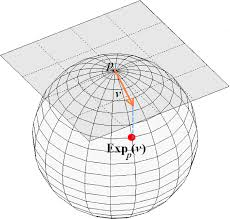
\includegraphics[width=0.35\columnwidth]{sphereMap}
		\end{figure}
	
	\noindent In the image we see that the exponential map is sending velocity vectors from $T_pS$ at the north pole to geodesics on the sphere $S^2$. Since the exponential map takes vectors in the tangent plane as arguments we can identify the argument of $exp_p$ in $\sigma(r,\theta)$ as the description of general vector of magnitude $r$ in direction $\cos\theta e_1 + \sin\theta e_2$ which starts at p. \\ 
	
	\noindent From class we known that all of the geodesics of the sphere must be great circles. Thus all we need is to translate this into a map that defines every point of the sphere in terms of great circles. First note that under this map we have that
		\begin{align*}
			\gamma_{e_1} &= (\sin r, 0, \cos r) \\ 
			\gamma'_{e_1} &= (\cos r, 0, -\sin r) \\ 
			\Rightarrow \gamma_{e_1}(0) &= (0,0,1) = p \\ 
				\gamma'_{e_1}(0) &= (1,0,0) = e_1
 		\end{align*}
	\noindent is the great circle beginning at point p and in direction of $v=e_1$. Thus we can re-write this same surface chart using this curve as a surface of revolution if we restrict $r\in(0, \pi)$:
		\begin{equation*}
			\sigma(r,\theta) = (\cos\theta\sin r, \sin\theta \sin r, \cos r)
		\end{equation*}
	Furthermore, if we allow $\theta = \pi/2$ then we see that our great circle becomes: 
		\begin{align*}
			\sigma(r, \pi/2) &= (0, \sin r, \cos r) \\ 
			\sigma'(r, \pi/2) &= (0, \cos r, -\sin r)\\ 
			\Rightarrow \sigma(0, \pi/2) &= (0, 0, 1) = p \\ 
				\sigma'(0, \pi/2) &= (0, 1, 0) = e_2 
		\end{align*}
	So to summarize, if we choose a magnitude for our velocity then we can choose a direction by specifying $\theta$ which is just the direction of $v$ in the tangent plane. This just recovers the standard spherical coordinates chart from way back in chapter 3 (page 130). 
\subsection*{Tapp 5.25}
	\textit{In Fig. 5.4 on page 252, the purple geodesic is asymptotic to the light-blue latitudinal curve.
		\begin{enumerate}
			\item Prove that a geodesic on a surface of revolution could not be asymptotic to a latitudinal curve unless the latitudinal curve is itself a geodesic.
			\item Rigorously justify the assertions in the discussion of Fig. 5.4
			\item Let $\gamma:\mathbb{R}\rightarrow S$ be a geodesic in the paraboloid 
				$$ S = \{(x,y,z)\in\mathbb{R}^3 | z = x^2 + y^2\} $$
			Prove that the height function, $h(x,y,z)=z$, composed with $\gamma$ has exactly one critical point $t_0$; it is decreasing on $(-\infty, t_0)$ and increasing on $(t_0, \infty)$. 
		\end{enumerate}	
	}
	\subsubsection*{1}
	Let $\beta(s)$ be a geodesic in S, a surface of revolution. By Clairaut's theorem we have that $\rho(s)\sin\psi(s) = \text{constant}$ where $\rho$ is the distance to the axis of rotation (z) and $\psi$ is the angle created between the velocity of the geodesic $\beta'(s)$ and the longitudinal curve through $\beta(s)$. \\
	
	\noindent From our last homework we have that if a latitude is a geodesic, then $x'(s) = \rho'(s) = 0$. Thus if $\beta$ approaches some other latitude asymptotically then we have that: 
		\begin{equation*}
			\rho\sin\psi = \text{constant} \neq 0
		\end{equation*}
	
	But taking the derivative of this equation with respect to s yields:\
		\begin{align*}
			\rho'\sin\psi &+ \rho\cos\psi \psi' = 0 \\ 
			\rho'\sin\psi &= -\rho\cos\psi \psi' 
		\end{align*}
	For latitudes $\psi = \frac{\pi}{2}$ which means that $\cos\psi \mapsto 0$ and $\sin\psi \mapsto 1$, thus: 
		\begin{align*}
			\rho' = 0
		\end{align*}
	We have a contradiction. $\rho'$ can't be zero because if our latitude isn't a geodesic then the latitude does not occur at an extreme value of $\rho$. Thus we have shown that a geodesic on a surface of revolution can't be asymptotic to a latitude unless that latitude is itself a geodesic. \qed 
	\subsubsection*{2}
		\begin{figure}[!hbt]
			\centering
			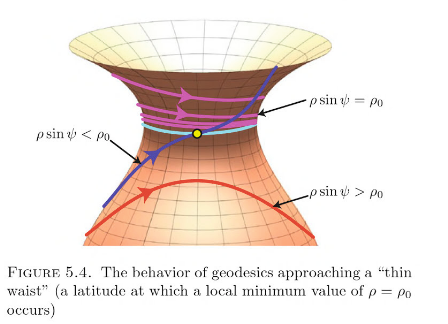
\includegraphics[scale = 0.75]{5-4}		
		\end{figure}
	
	\noindent For 2, we have that there are three cases $\rho\sin\psi = \rho_0$ (asymptote),  $\rho\sin\psi < \rho_0$ (passes through) and  $\rho\sin\psi > \rho_0$ (turns around). \\
	
	\noindent For the red curve, if the constant for Clairaut's theorem is $\rho\sin\psi> \rho_0$. We know that $\rho$ is decreasing because $\rho_0$ is a local minimum and so in order for the constant to remain greater than $\rho_0$, when $\sin\psi$ is 1,  $\rho > \rho_0$. Beyond this point, the sine function decreases. Therefore for our constant to remain greater than $\rho_0$ the function must turn because if $\sin\psi$ decreases, $\rho$ must increase to maintain our constant.  \\
	
	
	\noindent For the middle case (dark blue curve) where where $\rho\sin\psi < \rho_0$ we have that when $\rho = \rho_0$, $\sin\psi$ must be less than 1 in order to maintain the constant. Thus the velocity of this geodesic has a component that is perpendicular to the latitude and so it passes through the thin waist (the curve most follow the velocity). After passing through this point, $\rho$ begins to increase as the curve moves from the latitude and therefore, in order to maintain that the constant as less than $\rho_0$, $\sin\psi$ has to decrease. This is why the curve bends towards the longitude after it passes through the thin waist. \\
	
	\noindent Finally, for the case where $\rho\sin\psi = \psi_0$ (lavender curve) we have that $\rho$ must be decreasing as we approach the thin waist and therefore $\sin\psi$ must increase. $\psi=\frac{\pi}{2}$ can never be attained however as this would mean we have two geodesics that pass through the same point with velocity in the same direction. This contradicts the uniquely minimizing property of geodesics given by Theorem 5.19 and therefore indicates that curves satisfying this condition must asymptotically approach the \textit{thin waist}, never actually reaching $\psi = \pi/2$.  
	
	\subsubsection*{3}
	Consider the parabola of revolution generated by the curve $\gamma(t) = (t, 0 , t^2)$. This results in a surface patch that looks like: 
		\begin{equation*}
			\sigma(\theta, t) = (t\cos\theta, t\sin\theta, t^2) 
		\end{equation*}
	Now let's show that the curvature of this surface must always be positive... 
		\begin{align*}
			\sigma_\theta(\theta,t) &= (-t\sin\theta, t\cos\theta, 0) \\ 
			\sigma_{\theta,\theta}(\theta,t)&= (-t\cos\theta, -t\sin\theta, 0) \\ 
			\sigma_{t}(\theta, t) &= (\cos\theta, \sin\theta, 2t) \\ 
			\sigma_{tt}(\theta, t) &= (0 , 0, 2)\\ 
			\sigma_{\theta,t}(\theta, t) &= \sigma_{t,\theta} = (-\sin\theta, \cos\theta, 0) \\ 
			\sigma_\theta \times \sigma_t &= (2t^2\cos\theta, 2t^2\sin\theta, -t) \\
			|\sigma_\theta \times \sigma_t| &= v\sqrt{4t^2+1} \\ 
			N &= \frac{1}{\sqrt{4t^2+1}}(2t\cos\theta, 2t\sin\theta, -1) \\ 
			\Rightarrow E &= t^2, \quad F= 0, \quad G = 1+4t^2 \\ 
			e &= -\frac{-2t^2}{\sqrt{4t^2+1}}, \quad f = 0, \quad g = \frac{-2}{\sqrt{4t^2+1}} \\ 
			\Rightarrow K &= \frac{eg-f^2}{EG-F^2} = \frac{4t^2/(4t^2+1)}{t^2(4t^2+1)} = \frac{4}{(4t^2+1)^2} >0 \quad \forall t\\
		\end{align*}
	Thus our curvature is greater than zero. Admittedly I'm not sure how this helps us but I thought it would be helpful so I have calculated it. Now consider the family of curves $\beta(s)$ in the paraboloid which may be written by parametrizing our surface patch by s.
		\begin{equation*}
			\beta(s) = \sigma(\theta(s), t(s)) = (t(s)\cos\theta(s), t(s)\sin\theta(s), t(s)^2) 
		\end{equation*}
	The height function composed with all such curves returns: 
		\begin{align*}
			h\circ\beta(s) &= t(s)^2 \\ 
			\Rightarrow \frac{d}{ds}(h\circ\beta) &= 2t(s)t'(s) 
		\end{align*}

	\noindent Now there are a two cases to consider. The first case is for the longitudinal geodesics which are not allowed by this surface patch to go through the origin as that would require $t=0$ which can't happen for a surface of revolution (i.e. distance to axis of revolution must be greater than 0). If we instead used a different patch which allowed longitudes to extend through the origin then the trace of such geodesics would form the graph of a parabola in height. This would imply by simply differentiation that not only does such a curve have one critical point but that it is also concave up as required by the second and third conditions.\\ 
	
	\noindent The more difficult case is for geodesics which are not longitudes. We know that these geodesics can not be latitudes because the only latitude with $t'(s) = 0$ would be the point at the origin which is not included in this patch. From the derivative of the composition we have that the height of the geodesic will have a critical point $t_c$ if and only if $t'(s) = 0$ has a solution, $s_c$. For the case of inflection points, the only choice would be to have both an inflection point in height and in distance to the origin because we are on the paraboloid. By Clairaut's theorem though, this is impossible. Imagine approaching an inflection point in height and distance from \textit{above}. This would mean that your distance is decreasing until you reach $\sin\psi = 1$ because to have a critical point in height, the height is not changing and therefore the velocity vector of the geodesic must point along the longitude. After passing through this point though, both $\rho$ and $\sin\psi$ would decrease and there would be no way to maintain the constant for Clairaut's relation. The same argument applies to approaching from below except that after passing through the  inflection point, the curve would have both $\rho$ and $\sin\psi$ increasing which is also impossible. This means we only need to consider maxima and minima, not inflection points giving us 4 possible conclusions:
		\begin{enumerate}
			\item $t_c$ is a local minimum of the composition with h and $s_c$ is a local minimum of $t(s)$, the distance to the axis. 
			\item $t_c$ is a local maximum of the composition with h and $s_c$ is a local minimum of $t(s)$, the distance to the axis.
			\item $t_c$ is a local minimum of the composition with h and $s_c$ is a local maximum of $t(s)$, the distance to the axis.
			\item $t_c$ is a local maximum of the composition with h and $s_c$ is a local maximum of $t(s)$, the distance to the axis.
		\end{enumerate}
	\noindent Now for case 2 where we have a minimum of distance to the axis, changing s would increase $t(s)$ i.e. $t(s)>t(s_c)=t_0$ for $s\neq s_c$. Since our height depends on $t^2$ we can't also have a minimum of height because increasing s increases t which increases the height. For case three the exact opposite argument applies because having a maximum in $t(s)$ means that any other $s$ than $s_c$ would have a shorter distance do the axis and therefore $t(s)<t(s_c)=t_c$ which doesn't make sense because our surface is a paraboloid. For 4, we have that both the distance and height are maximized. This seems reasonable for a general curve in the paraboloid but we must show that this is impossible for a geodesic. The only options for a maximum in height are to approach it from below. Thus after passing through the point we have the same issue as with the inflection point because at the maximum we have that $\sin\psi$ and $\rho$ are maximized and so moving down would have both $\rho$ and $\sin\psi$ decrease which makes it impossible to maintain $\rho\sin\psi=$ constant.  Thus the only choice is 1.\\
	
	\noindent Choice 1 works because for a minimum in height and distance to the origin, the only choice is for the geodesic to approach this critical point from above. This satisfies $\rho$ is decreasing and $\sin\psi$ is increasing towards 1. At the critical point $\sin\psi$ is maximized and so afterwards, where the curve goes up, we have that $\rho$ is increasing and $\sin\psi$ must decrease. This makes it possible for only this curve to satisfy Clairaut's relation. \\ 
	
	\noindent Now we have shown that any critical point must be a local minimum in height and I must convince you that there can be no other critical points. From my previous argument the only choice for another such point would be a local minimum in height and distance to the axis of rotation. This is impossible though, (following Steve's argument from last week) as the extreme value theorem would necessitate having a local maximum of height between two minima. Thus there can only be one critical point.\\ 
	
	\noindent Lastly,  because we have only one critical point that is a minimum of height, it must be true that the geodesic is concave up, satisfying the secondary conditions that the geodesics's height is increasing as $t\in (t_c, \infty)$ and decreasing on $(-\infty, t_c)$. Thus we have shown that any geodesic of the paraboloid must have exactly one critical point in height which and appear concave up. \qed 
	 
	
	
	
	
	
	
	
\end{document}




































